\chapter{Analyse}
\label{chap:analyse}
Dans ce chapitre, nous allons dans une première partie, étudier la stabilité de nos différentes modélisations (espace d'état d'ordre 4, 3 et 2), puis leurs commandabilités et observabilités. Dans une seconde partie, nous étudierons les performances dynamiques des différents modèles à travers une analyse temporelles et fréquentielle. Dans l'ensemble du chapitre sera abordé l'impact des simplifications effectués sur les modèles espace d'état d'ordre 3 et 2.
Comme nous souhaitons asservir le procédé en vitesse et non en position, nous étudierons la sortie de performance $V_g(t)$ des modèles  et non $V_s(t)$. 

\section{Analyse des modèles}
\subsection{Stabilité}
Nous avons décidé d'étudier la stabilité asymptotique afin de savoir si l'ensemble des états de nos modèles sont stables et non uniquement ceux qui sont observables comme en stabilité BIBO. \\

\noindent Les valeurs propres de notre système d'ordre 4 sont : (calculé à l'aide de matlab)\\
\begin{equation}
{0 ; -132749,8861 ; -4,0655 ; -7748,0483 }
\end{equation}
Nous remarquons que les valeurs propres sont toutes à partie réelle négatives, le système d'ordre 4 est donc asymptotiquement stable.

\noindent Les valeurs propres de notre système d'ordre 3 sont : (calculé à l'aide de matlab)\\
\begin{equation}
{ 0 ; -7748,0484 ; -3,9516 }
\end{equation}
Nous remarquons que les valeurs propres sont toutes à parties réelles négatives, le système d'ordre 3 est donc asymptotiquement stable.\\

C'était prévisible car le modèle d'ordre 3 est une simplification du modèle d'ordre 4, qui est stable. Nous remarquons aussi que la troisième valeur propre du système d'ordre 3, qui normalement doit être similaire à la troisième valeur propre du système d'ordre 4 a légèrement variée. Cette différence est une première conséquence de la perte d'une dynamique engendrée par la simplification.

\noindent Les valeurs propres de notre système d'ordre 2 sont : (calculé à l'aide de matlab)\\
\begin{equation}
{0 ; -3,9506 }
\end{equation}
Nous remarquons que les valeurs propres sont toutes à parties réelles négatives, le système d'ordre 2 est donc asymptotiquement stable.\\
Comme précédemment, cette conclusion était prévisible, néanmoins on remarque une autre conséquence de la simplification sur la seconde valeur propre qui est légèrement différente de celle du modèle d'ordre 3.

\subsection{Commandabilité}
L'étude de la commandabilité d'un système nous permettra de savoir quels états sont commandables, c'est à dire qu'il sera possible de modifier la dynamique qu'ils représentent par un asservissement. Cette étude se fera uniquement sur l'espace d'état d'ordre 4 car les deux autres modèles découlent de celui-ci. Un système (sous forme d'espace d'état) est commandable, d'après le critère de Kalman, si 
la matrice de commandabilité $\mathcal{C}_m$ est de rang plein donc égale à la dimension de A.\\

Où, $ \mathcal{C}_m = \begin{bmatrix} B  & AB & \dots & A^{n−1}B\end{bmatrix}$
Nous avons étudié la commandabilité sur matlab et le résultat est que :
$$rang(\mathcal{C}_m) = n = 4 $$
Donc le système est commandable. Cela nous permet de mettre en place un retour d'état. 

\subsection{Observabilité}
L'étude de l'observabilité d'un système nous permettra de savoir quels états sont observables, c'est à dire s'il est possible de déterminer la valeur des états à partir de mesures de la sortie. Cette étude se fera uniquement sur l'espace d'état d'ordre 4 car les deux autres modèles découlent de celui-ci. Un système (sous forme d'espace d'état) est observable, d'après le critère de Kalman, si 
la matrice d'observabilité  $\mathcal{O}$ est de rang plein donc égale à la dimension de A.\\

Où, $ \mathcal{O} = \begin{bmatrix} C \\ CA \\ \vdots \\ CA^{n−1} \end{bmatrix}$
Nous avons étudié l'observabilité sur matlab et le résultat est que :
$$rang(\mathcal{O}) = dim(A)=4 $$
Donc le système est observable, néanmoins intuitivement ce résultat semble faux.

\section{Analyse temporelle et fréquentielle}
Nous avons étudié les performances de nos modèles grâce à deux types de réponses : 
\begin{itemize}
\item Une réponse à un échelon unité (voir figure \ref{fig:echelon}).
\item Une réponse fréquentielle représentée par un diagramme de Bode (voir figure \ref{fig:bode}).
\end{itemize}

\begin{figure}[!ht]
\centering
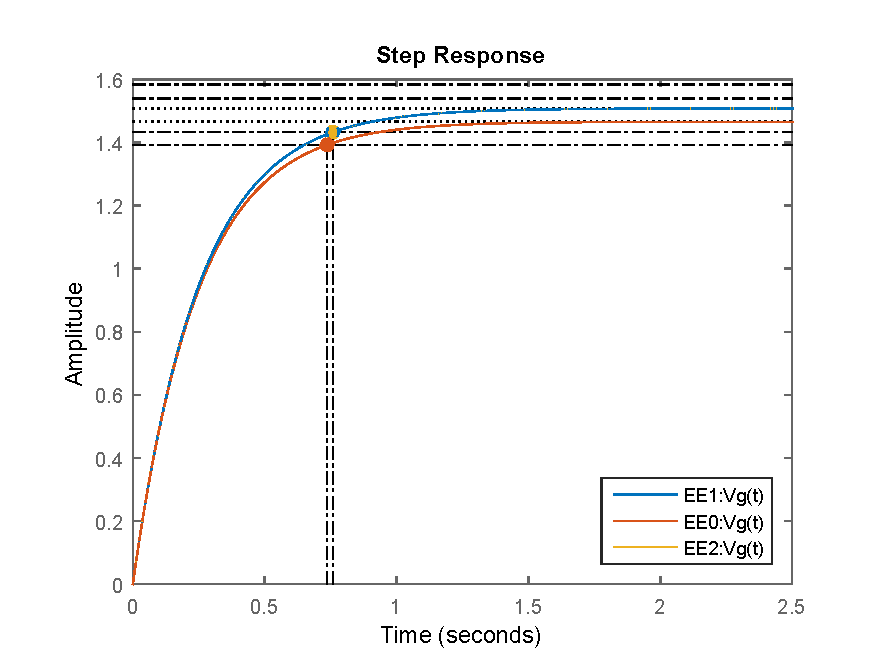
\includegraphics[width=.8\textwidth]{./II/images/echelon.pdf}
\caption{\label{fig:echelon}Réponse à un échelon unité de $V_g(t)$ des modèles EE0, EE1 et EE2.}
\end{figure}
\begin{figure}[!ht]
\centering
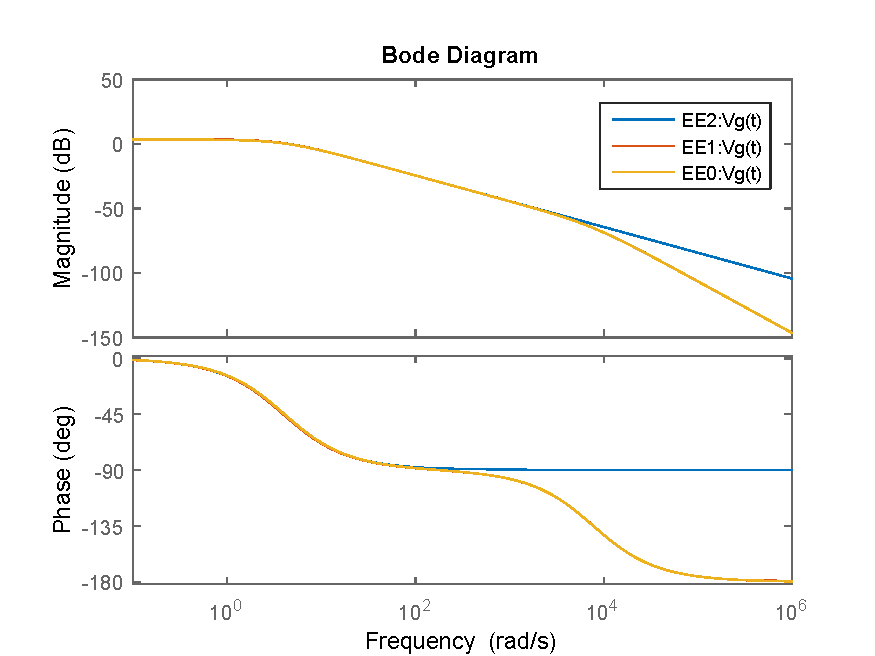
\includegraphics[width=.8\textwidth]{./II/images/bode.pdf}
\caption{\label{fig:bode}Diagramme de Bode sur $V_g(t)$ des modèles EE0, EE1 et EE2.}
\end{figure}

\subsection{Performances Statiques}
Nous étudions $V_g(t)$ en temps que sortie de performance (figure \ref{fig:echelon}).\\
Nos modèles présentent des gains statiques qui varient d'un modèle à l'autre, à cause des simplifications : \\

\noindent Gain statique de EE0 : $1,4658$\\

\noindent Gain statique de EE1 : $1.5080$\\

\noindent Gain statique de EE0 : $1.5080$\\

On peut constater qu'entre le modèle EE0 et le modèle EE1, il y a une erreur de $0.0423$ et qu'en le modèle EE1 et le modèle EE2 l'erreur vaut $2.0241*10^{-8}$. La première simplification engendre une erreur d'environ $2\%$ et la suivante de le l'ordre de $10^{-8}\%$. L'asservissement risquera donc de présenter une erreur statique causée par ces simplifications.

\subsection{Performances dynamiques}
Nous étudions $V_g(t)$ en temps que sortie de performance (figure \ref{fig:echelon}).\\
Nous avons choisis d'étudier le temps de montée, le temps de réponse et le dépassement car ce sont des paramètres précis et déterminants en terme de performances. 

\noindent Temps de montées :\\
\noindent Sur EE0 : 0.5404s \\
\noindent Sur EE1 : 0.5560s\\
\noindent Sur EE2 : 0.5561s\\
\noindent Erreur de EE0 à EE1 : 0.0156 s (2.8826$\%$)\\
\noindent Erreur de EE1 à EE2 : 1.3830e-04 s(0.0249$\%$)\\
Nous pouvons remarquer que le temps de montée est aux alentours d'une demie seconde. Les différences entre les temps de montées des différents modèles risquent de créer une erreur sur l'asservissement, en effet elle témoigne d'une différence dans les dynamiques des modèles (ce qui est une conséquence logique de la simplification). Le test de la commande sur EE0 risque de démontrer une erreur dynamique.\\

 
\noindent Temps de réponses à $5\%$ :\\
\noindent Sur EE0 : 0.7370 s\\
\noindent Sur EE1 : 0.7582 s\\
\noindent Sur EE2 : 0.7583 s\\
\noindent Erreur de EE0 à EE1 : 0.0212 s (2.8821$\%$)\\
\noindent Erreur de EE1 à EE2 : 5.9211e-05 s(7.8089e-05$\%$)\\
Comme pour la performance précédente , la valeur du temps de réponse varie et cela entrainera de potentielles erreurs d'asservissement.

\noindent Dépassements  :\\
Le modèle en boucle ouverte ne présente pas de dépassement.
\subsection{Analyse fréquentielle}
On peut remarquer sur le diagramme de Bode, figure \ref{fig:bode}, qu'il y a une compensation pôle zéro dans le modèle EE0 car nous avons uniquement trois changements d'allures. Cela se confirme sur une vue des pôles et des zéros sur un plan complexe (voir figure \ref{fig:poles}) ou une fonction de transfert. Cette figure met en évidence la compensation d'un pôle électrique qui agis à haute fréquence. Sur le diagramme de Bode, nous pouvons aussi constater que les modèles semblent avoir des réponses fréquentielles assez similaires. On peut aussi voir l'absence de la dernière dynamique de EE2 due à la simplification.

\begin{figure}[!ht]
\centering
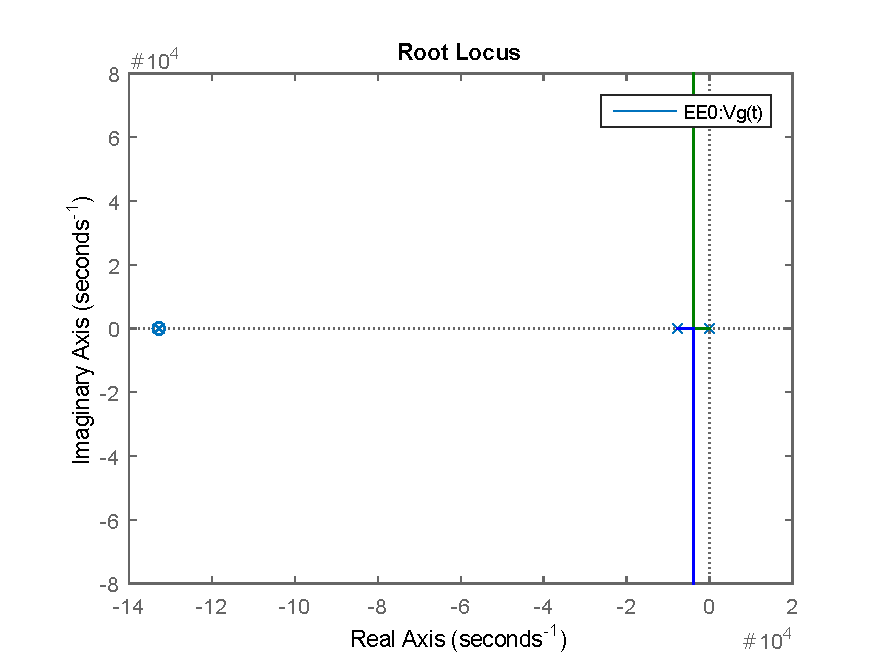
\includegraphics[width=.5\textwidth]{./II/images/poles.pdf}
\caption{\label{fig:poles}Pôles et zéros dans le plan complexe du transfert vers $V_g(t)$ du modèles EE0.}
\end{figure}